\documentclass[submit]{harvardml}

\course{CS181-S22}
\assignment{Assignment \#1}
\duedate{7:59pm ET, February 4, 2022} 

\usepackage[OT1]{fontenc}
\usepackage[colorlinks,citecolor=blue,urlcolor=blue]{hyperref}

\usepackage[pdftex]{graphicx}
\usepackage{graphicx}
\graphicspath{ {./} }

\usepackage{caption}
\usepackage{fullpage}
\usepackage{soul}
\usepackage{amsmath}
\usepackage{amssymb}
\usepackage{color}
\usepackage{todonotes}
\usepackage{listings}
\usepackage{common}
\usepackage{framed}

\usepackage[mmddyyyy,hhmmss]{datetime}

\definecolor{verbgray}{gray}{0.9}

\lstnewenvironment{csv}{
  \lstset{backgroundcolor=\color{verbgray},
  frame=single,
  framerule=0pt,
  basicstyle=\ttfamily,
  columns=fullflexible}}{}
 

\begin{document}
\begin{center}
{\Large Homework 1: Regression}\\
\end{center}

\subsection*{Introduction}
This homework is on different forms of linear regression and focuses
on loss functions, optimizers, and regularization. Linear regression
will be one of the few models that we see that has an analytical
solution.  These problems focus on deriving these solutions and
exploring their properties.

If you find that you are having trouble with the first couple
problems, we recommend going over the fundamentals of linear algebra
and matrix calculus (see links on website).  The relevant parts of the
\href{https://github.com/harvard-ml-courses/cs181-textbook/blob/master/Textbook.pdf}{cs181-textbook notes are Sections 2.1 - 2.7}.  We strongly recommend
reading the textbook before beginning the homework.

    We also encourage you to first read the \href{http://users.isr.ist.utl.pt/~wurmd/Livros/school/Bishop\%20-\%20Pattern\%20Recognition\%20And\%20Machine\%20Learning\%20-\%20Springer\%20\%202006.pdf}{Bishop textbook}, particularly:
Section 2.3 (Properties of Gaussian Distributions), Section 3.1
(Linear Basis Regression), and Section 3.3 (Bayesian Linear
Regression). (Note that our notation is slightly different but the
underlying mathematics remains the same!).

\textbf{Please type your solutions after the corresponding problems using this
\LaTeX\ template, and start each problem on a new page.} You may find
the following introductory resources on \LaTeX\ useful: 
\href{http://www.mjdenny.com/workshops/LaTeX_Intro.pdf}{\LaTeX\ Basics} 
and \href{https://www.overleaf.com/learn/latex/Free_online_introduction_to_LaTeX_(part_1)}{\LaTeX\ tutorial with exercises in Overleaf}

Homeworks will be submitted through Gradescope. You will be added to
the course Gradescope once you join the course Canvas page. If you
haven't received an invitation, contact the course staff through Ed.

\textbf{Please submit the writeup PDF to the Gradescope assignment
  `HW1'.} Remember to assign pages for each question.

\textbf{Please submit your \LaTeX file and code files to the
  Gradescope assignment `HW1 - Supplemental'.} Your files should be
named in the same way as we provide them in the repository,
e.g. \texttt{T1\_P1.py}, etc.


%%%%%%%%%%%%%%%%%%%%%%%%%%%%%%%%%%%%%%%%%%%%%
% Problem 1
%%%%%%%%%%%%%%%%%%%%%%%%%%%%%%%%%%%%%%%%%%%%%

\begin{problem}[Optimizing a Kernel, 15pts]

Kernel-based regression techniques are similar to nearest-neighbor
regressors: rather than fit a parametric model, they predict values
for new data points by interpolating values from existing points in
the training set.  In this problem, we will consider a kernel-based
regressor of the form:
\begin{equation*}
  f(x^*) = \sum_{n} K(x_n,x^*) y_n 
\end{equation*}
where $(x_n,y_n)$ are the training data points, and $K(x,x')$ is a
kernel function that defines the similarity between two inputs $x$ and
$x'$. Assume that each $x_i$ is represented as a column vector, i.e. a
$D$ by 1 vector where $D$ is the number of features for each data
point. A popular choice of kernel is a function that decays as the
distance between the two points increases, such as
\begin{equation*}
  K(x,x') = \exp\left(\frac{-||x-x'||^2_2}{\tau}\right) = \exp\left(\frac{-(x-x')^T (x-x')}{\tau} \right) 
\end{equation*}
where $\tau$ represents the square of the lengthscale (a scalar value).  In this
problem, we will consider optimizing what that (squared) lengthscale
should be.

\begin{enumerate}

\item Let $\{(x_n,y_n)\}_{n=1}^N$ be our training data set.  Suppose
  we are interested in minimizing the residual sum of squares.  Write
  down this loss over the training data $\mcL(W)$ as a function of $\tau$.

  Important: When computing the prediction $f(x_i)$ for a point $x_i$
  in the training set, carefully consider for which points $x'$ you should be including
  the term $K(x_i,x')$ in the sum.

\item Take the derivative of the loss function with respect to $\tau$.
\end{enumerate}

\end{problem}


\newpage

\begin{framed}
\noindent\textbf{Problem 1} (cont.)\\

\begin{enumerate}
\setcounter{enumi}{2}
\item Consider the following data set:
\begin{csv}
  x , y
  0 , 0
  1 , 0.5
  2 , 1
  3 , 2
  4 , 1
  6 , 1.5
  8 , 0.5 
\end{csv}
And the following lengthscales: $\tau=.01$, $\tau=2$, and $\tau=100$.

Write some Python code to compute the loss with respect to each kernel
for the dataset provided above. Which lengthscale does best?  
For this problem, you can use our staff \textbf{script to compare your
  code to a set of staff-written test cases.} This requires, however,
that you use the structure of the starter code provided in
\texttt{T1\_P1.py}. More specific instructions can be found at the top
of the file \texttt{T1\_P1\_Testcases.py}. You may run the test cases
in the command-line using \texttt{python T1\_P1\_TestCases.py}.
\textbf{Note that our set of test cases is not comprehensive: just
  because you pass does not mean your solution is correct! We strongly
  encourage you to write your own test cases and read more about ours
  in the comments of the Python script.}
  
\item Plot the function $(x^*, f(x^*))$ for each of the
  lengthscales above.  You will plot $x^*$ on the x-axis and the
  prediction $f(x^*)$ on the y-axis.  For the test inputs $x^*$, you
  should use an even grid of spacing of $0.1$ between $x^* = 0$ and
  $x^* = 12$.  (Note: it is possible that a test input $x^*$ lands
  right on top of one of the training inputs above.  You can still use
  the formula!) 

  Initial impressions: Briefly describe what happens in each of the
  three cases.  Is what you see consistent with the which lengthscale
  appeared to be numerically best above?  Describe why or why not.

\item Bonus: Code up a gradient descent to optimize the kernel for the
  data set above.
  Start your gradient descent from $\tau=2$. Report on what you
  find.\\\\

  Note: Gradient descent is discussed in Section 3.4 of the
  cs181-textbook notes and Section 5.2.4 of Bishop, and will be
  covered later in the course!

\end{enumerate}

\end{framed}  


\newpage
\subsubsection*{Solution}

\begin{enumerate}

\item 

\begin{equation*}
\mcL(W) = \sum_{i} (y_i - f(x_i))^2
\end{equation*}

In calculating $f(x_i)$, we don't include $K(x_i, x_i)y_n$ as $x_i$ is the value whose
target we are predicting

\begin{equation*}
= \sum_{i} \left(y_i - \sum_{n\neq i} K(x_n, x_i) y_n \right)^2 
\end{equation*}


\begin{equation*}
\mcL(W) = \sum_{i} \left(y_i - \sum_{n\neq i} \exp\left(\frac{-(x_n-x_i)^T (x_n-x_i)}{\tau} \right) y_n\right)^2 
\end{equation*}

\item 

\begin{equation*}
\frac{d}{d\tau}  \mcL(W)  = 
\frac{d}{d\tau} \left( \sum_{i} \left(y_i - \sum_{n\neq i} K(x_n, x_i) y_n \right)^2 \right)
\end{equation*}

\begin{equation*}
=  \sum_{i}  2 \left(y_i - \sum_{n\neq i} K(x_n, x_i) y_n \right) 
\left(- \sum_{n\neq i}  \frac{d}{d\tau} \left( K(x_n, x_i) \right) y_n \right) 
\end{equation*}


\begin{multline*}
=  
\sum_{i}  - 2 \left(y_i - \sum_{n\neq i} \exp\left(\frac{-(x_n-x_i)^T (x_n-x_i)}{\tau} \right) y_n\right) \\
\left( \sum_{n\neq i} \left(\frac{(x_n-x_i)^T (x_n-x_i)}{\tau^2} \right) \exp\left(\frac{-(x_n-x_i)^T (x_n-x_i)}{\tau} \right)  y_n\right) 
\end{multline*}

\item

Computed using the script in T1\_P1.py, the loss for $\tau=0.01$ is 8.75, $\tau=2$ is 3.30501649457,
and $\tau=100$ is 120.359193422. 

\newpage
\item 

The following plot is made in the script T1\_P1.py.

\begin{figure}[h]
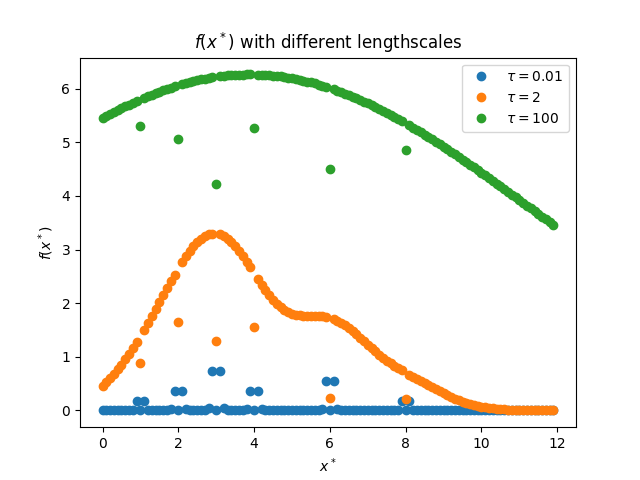
\includegraphics[scale=0.8]{P1}
\centering
\end{figure}

In the case of $\tau=0.01$, since $f(x^*)$ is not normalized, each of the $K(x_n, x_*)$ weights
is much closer to 1 and the overall prediction is much greater than for the other two values of 
$\tau$. Additionally, target values for data points farther away from the one being 
predicted are weighted too heavily, resulting in a not-too-fine fit for the data.

In the case of $\tau=100$, values that are not exactly that which is being predicted are almost
not taken account of (e.g. have very minimal weight) and so the prediction is almost zero except 
for $x$ values that happen to be very similar to those in the training set.

In the case of $\tau=2$, training set values similar to the value for which $y$ is being predicted
are weighted enough that $x$ values not similar to one of the training set points (e.g.
2.5, which is right in between its closest training set values 2 and 3) do have meaningful
predictions. They are not weighted so much that closeness is not sufficiently taken account for,
however.



\end{enumerate}

\newpage







%%%%%%%%%%%%%%%%%%%%%%%%%%%%%%%%%%%%%%%%%%%%%
% Problem 2
%%%%%%%%%%%%%%%%%%%%%%%%%%%%%%%%%%%%%%%%%%%%%

\begin{problem}[Kernels and kNN, 10pts]

Now, let us compare the kernel-based approach to an approach based on
nearest-neighbors.  Recall that kNN uses a predictor of the form
  \begin{equation*}
    f(x^*) = \frac{1}{k} \sum_n y_n \mathbb{I}(x_n \texttt{ is one of k-closest to } x^*)
  \end{equation*}

\noindent where $\mathbb{I}$ is an indicator variable. For this problem, you will use the \textbf{same dataset and kernel as in Problem 1}.


For this problem, you can use our staff \textbf{script to compare your code to a set of staff-written test cases.} This requires, however, that you use the structure of the starter code provided in \texttt{T1\_P2.py}. More specific instructions can be found at the top of the file \texttt{T1\_P2\_Testcases.py}. You may run the test cases in the command-line using \texttt{python T1\_P2\_TestCases.py}.
\textbf{Note that our set of test cases is not comprehensive: just because you pass does not mean your solution is correct! We strongly encourage you to write your own test cases and read more about ours in the comments of the Python script.}

\vspace{0.5cm}
\noindent\emph{Make sure to include all required plots in your PDF.}


\begin{enumerate}

\item Implement kNN for $k=\{1, 3, N-1\}$ where N is the size of the dataset, then plot the results for each $k$. To find the distance between points, use the kernel function from Problem 1 with lengthscale $\tau=1$. 

As before, you will plot $x^*$ on the x-axis and the prediction $f(x^*)$ on the y-axis.  For the test inputs $x^*$, you should use an even grid of spacing of $0.1$ between $x^* = 0$ and $x^* = 12$.  (Like in Problem 1, if a test point lies on top of a training input, use the formula without excluding that training input.)
  
  You may choose to use some starter Python code to create your plots
  provided in \verb|T1_P2.py|.  Please \textbf{write your own
    implementation of kNN} for full credit.  Do not use external
  libraries to find nearest neighbors.
  
\item Describe what you see: What is the behavior of the functions in
  these three plots?  How does it compare to the behavior of the
  functions in the three plots from Problem 1?  Are there situations
  in which kNN and kernel-based regression interpolate similarly?
  Extrapolate similarly?  Based on what you see, do you believe there
  exist some values of $k$ and $\tau$ for which the kNN and kernel-based regressors produce the exact same classifier (ie. given \textit{any} point $x$, the two regressors will produce the same prediction $f(x)$)? Explain your answer.
  
\item Why did we not vary $\tau$ for the kNN approach?

\end{enumerate}

\end{problem}

\newpage
\subsubsection*{Solution}

\begin{enumerate}

\item This plot is generated in T1\_P2.py.

\begin{figure}[h]
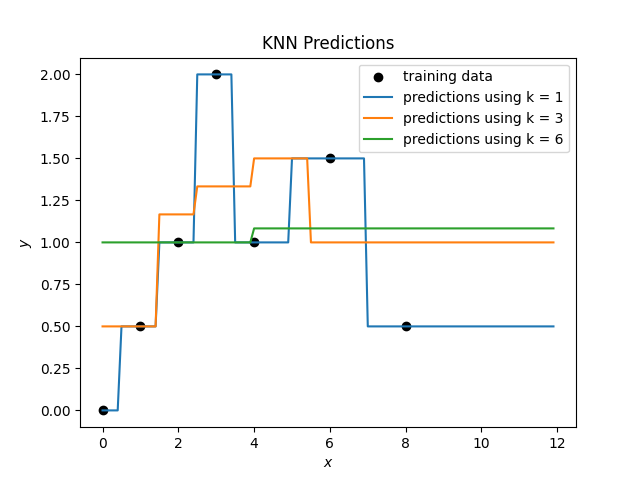
\includegraphics[scale=0.8]{P2}
\centering
\end{figure}

\item 

Depending on $K$, the functions in these plots either average out too large a sample of the 
training data, leading to a similar prediction across large ranges of $x$ (seen in the case of $k=6$), 
or predict by ``copying" the closest value in the training data (seen in the case of $x=1$). Setting
$x=3$ results in the best fit of the data, as it balances out these two negative aspects.

The biggest difference between this method and kernel regression is that the resulting predictions
change a lot more abruptly when crossing certain $x$ values. As for differing values of $K$ and $\tau$,
the effect of increasing $K$ had a similar effect to increasing $\tau$: training data points similar
to the $x^*$ being predicted were not sufficiently emphasized and the resulting prediction graph
was too ``flat." 

kNN and kernel-based regression both interpolate and extrapolate similarly in the case of large 
values of $K$ and $\tau$. In these cases, $x$ values in the training set that are too far away 
from the $x*$ whose target is being predicted are too greatly weighted.

Based on this, kNN and kernel-based regressors produce the exact same classifier when $k=N$ and 
$\tau$ approaches infinity (equally weighing every training data point). The same cannot be said
for $K=1$ and $\tau$ approaching 0, as kernel-based regression will only meaningfully weigh points 
in the training set if they exactly match that which is being predicted for.

\item 

$\tau$ was not varied for this approach as changing it would have no effect on which points
would be calculated to be nearest to a point. It only made sense to vary $\tau$ in the kernel
regression approach as the magnitude of closeness was relevant. In kNN, only the relative closeness
is relevant and this relative closeness does not change with different values of $\tau$.

\end{enumerate}


\newpage 

%%%%%%%%%%%%%%%%%%%%%%%%%%%%%%%%%%%%%%%%%%%%%
% Problem 3
%%%%%%%%%%%%%%%%%%%%%%%%%%%%%%%%%%%%%%%%%%%%%

\begin{problem}[Deriving Linear Regression, 10pts]

  The solution for the least squares linear regressions ``looks'' kind
  of like a ratio of covariance and variance terms.  In this problem,
  we will make that connection more explicit. \\

  \noindent Let us assume that our data are tuples of scalars $(x,y)$ that are
  described by some joint distribution $p(x,y)$.  For clarification, the joint distribution $p(x,y)$ is just another way of saying the ``joint PDF'' $f(x,y)$, which may be more familiar to those who have taken Stat 110, or equivalent. \\
  
  \noindent We will consider the process of fitting these data from this distribution with the best linear model
  possible, that is a linear model of the form $\hat{y} = wx$ that
  minimizes the expected squared loss $E_{x,y}[ ( y - \hat{y} )^2
  ]$.\\

\noindent \emph{Notes:} The notation $E_{x, y}$ indicates an
expectation taken over the joint distribution $p(x,y)$.  Since $x$ and
$y$ are scalars, $w$ is also a scalar.
  
  \begin{enumerate}

  \item Derive an expression for the optimal $w$, that is, the $w$
    that minimizes the expected squared loss above.  You should leave
    your answer in terms of moments of the distribution, e.g. terms
    like $E_x[x]$, $E_x[x^2]$, $E_y[y]$, $E_y[y^2]$, $E_{x,y}[xy]$
    etc.

\item Provide unbiased and consistent formulas to estimate $E_{x, y}[yx]$
 and $E_x[x^2]$ given observed data $\{(x_n,y_n)\}_{n=1}^N$.

\item In general, moment terms like $E_{x, y}[yx]$, $E_{x, y}[x^2]$,
  $E_{x, y}[yx^3]$, $E_{x, y}[\frac{x}{y}]$, etc. can easily be
  estimated from the data (like you did above).  If you substitute in
  these empirical moments, how does your expression for the optimal
  $w^*$ in this problem compare with the optimal $w^*$ that we see in
  Section 2.6 of the cs181-textbook?

\item Many common probabilistic linear regression models assume that
  variables x and y are jointly Gaussian.  Did any of your above
  derivations rely on the assumption that x and y are jointly
  Gaussian?  Why or why not?
    
\end{enumerate}

\end{problem}

\newpage
\subsubsection*{Solution}

\begin{enumerate}

\item Let $\mcL(w)$ be the expected squared loss of the linear model given
the parameter $w$:

\begin{equation*}
    \mcL(w) = E_{x,y}[(y-\hat{y})^2]
\end{equation*}
\begin{equation*}
    = E_{x,y}[y^2 - 2y\hat{y} -\hat{y}^2]
\end{equation*}
\begin{equation*}
    = E_{x,y}[y^2] - 2E_{x,y}[y\hat{y}] - E_{x,y}[\hat{y}^2]
\end{equation*}
\begin{equation*}
    = E_{x,y}[y^2] - 2E_{x,y}[y(wx))] - E_{x,y}[(wx)^2]
\end{equation*}
\begin{equation*}
    = E_{x,y}[y^2] - 2wE_{x,y}[yx)] - w^2E_{x,y}[x^2]
\end{equation*}

This is a quadratic function of $w$, meaning we can find the optimal value $w*$
by differentiation:

\begin{equation*}
    \frac{d}{dw} \mcL(w) = -2E_{x,y} + 2wE_{x,y}[x^2]
\end{equation*}

Setting the equation to zero we have:

\begin{equation*}
    2E_{x,y} = 2w^*E_{x,y}[x^2]
\end{equation*}

\begin{equation*}
    w^* = \frac{E_{x,y}[xy]}{E_{x,y}[x^2]}
\end{equation*}

\item

Estimations of these moments can be gathered by averaging functions of
the observed data:

\begin{equation*}
    E_{x,y}[xy] = \frac{1}{N} \sum_n x_n y_n
\end{equation*}

\begin{equation*}
    E_{x,y}[x^2] = \frac{1}{N} \sum_n x_n^2
\end{equation*}


Substitution these estimations into the description of the optimal $w^*$ we have:

\begin{equation*}
    w^* = \frac{\frac{1}{N} \sum_n x_n y_n}{\frac{1}{N} \sum_n x_n^2}
    = \frac{\sum_n x_n y_n}{\sum_n x_n^2}
\end{equation*}

The definition of the optimal $w*$ from the textbook is the following:

\begin{equation*}
    w^* = (\mathbf{X}^\top \mathbf{X})^{-1} \mathbf{X}^\top \mathbf{y}
\end{equation*}

These two definitions are similar in the the inverse of the "square" of the
observed $x$-values is being multiplied by the product of the observed $x$-values 
and their targets $\mathbf{y}$.

\item

The derivations made did not rely on the assumption that $x$ and $y$ are jointly Gaussian.
This is because the derivation was a partial derivative in terms of $w$, meaning that changing 
the distribution of the variables would not have had an effect on the resulting derivation 
given that terms of the form $E_{x,y}[g(x,y)]$ were interpreted as constants.

\end{enumerate}


%%%%%%%%%%%%%%%%%%%%%%%%%%%%%%%%%%%%%%%%%%%%%
% Problem 4
%%%%%%%%%%%%%%%%%%%%%%%%%%%%%%%%%%%%%%%%%%%%%

\begin{problem}[Modeling Changes in Republicans and Sunspots, 15pts]
  
 The objective of this problem is to learn about linear regression
 with basis functions by modeling the number of Republicans in the
 Senate. The file \verb|data/year-sunspots-republicans.csv| contains the
 data you will use for this problem.  It has three columns.  The first
 one is an integer that indicates the year.  The second is the number
 of Sunspots observed in that year.  The third is the number of Republicans in the Senate for that year.
 The data file looks like this:
 \begin{csv}
Year,Sunspot_Count,Republican_Count
1960,112.3,36
1962,37.6,34
1964,10.2,32
1966,47.0,36
\end{csv}

You can see scatterplots of the data in the figures below.  The horizontal axis is the Year, and the vertical axis is the Number of Republicans and the Number of Sunspots, respectively.

\begin{center}
\includegraphics[width=.5\textwidth]{data/year-republicans}
\end{center}

\begin{center}
\includegraphics[width=.5\textwidth]{data/year-sunspots}
\end{center}

(Data Source: \url{http://www.realclimate.org/data/senators_sunspots.txt})\\
\vspace{-5mm}


\vspace{0.5cm}
\noindent\emph{Make sure to include all required plots in your PDF.}

\begin{enumerate}

\item In this problem you will implement ordinary least squares
  regression using 4 different basis functions for \textbf{Year
    (x-axis)} v. \textbf{Number of Republicans in the Senate
    (y-axis)}. Some starter Python code that implements simple linear
  regression is provided in \verb|T1_P4.py|.

  Note: The numbers in the \emph{Year} column are large (between $1960$ and $2006$), especially when raised to various powers. To avoid numerical instability due to ill-conditioned matrices in most numerical computing systems, we will scale the data first: specifically, we will scale all ``year'' inputs by subtracting $1960$ and then dividing by $40$. Similarly, to avoid numerical instability with numbers in the \emph{Sunspot\_Count} column, we will also scale the data first by dividing all ``sunspot count'' inputs by $20$. Both of these scaling procedures have already been implemented in lines $65-69$ of the starter code in \verb|T1_P4.py|. Please do \emph{not} change these lines!

First, plot the data and regression lines for each of the following sets of basis functions, and include
the generated plot as an image in your submission PDF. You will therefore make 4 total plots:
\begin{enumerate}
	\item[(a)] $\phi_j(x) = x^j$ for $j=1, \ldots, 5$\\
    ie, use basis $y = a_1 x^1 + a_2 x^2 + a_3 x^3 + a_4 x^4 + a_5 x^5$ for some constants $\{a_1, ..., a_5\}$. 
    \item[(b)] $\phi_j(x) = \exp{\frac{-(x-\mu_j)^2}{25}}$ for $\mu_j=1960, 1965, 1970, 1975, \ldots 2010$
	\item[(c)] $\phi_j(x) = \cos(x / j)$ for $j=1, \ldots, 5$
	\item[(d)] $\phi_j(x) = \cos(x / j)$ for $j=1, \ldots, 25$
\end{enumerate}
\vspace{-2mm}


{\footnotesize * Note: Please make sure to add a bias term for all your basis functions above in your implementation of the \verb|make_basis| function in \verb|T1_P4.py|.}
  
Second, for each plot include the residual sum of squares error. Submit the generated plot and residual sum-of-squares error for each basis in your LaTeX write-up.
\end{enumerate}

\end{problem}

\begin{framed}
\noindent\textbf{Problem 4} (cont.)\\
\begin{enumerate}
\setcounter{enumi}{1}
\item Repeat the same exact process as above but for \textbf{Number of Sunspots (x-axis)} v. \textbf{Number of Republicans in the Senate (y-axis)}. 
Now, however, only use data from before 1985, and only use basis functions (a), (c), and (d) -- ignore basis (b). You will therefore make 3 total plots. For each plot make sure to also include the residual sum of squares error.



Which of the three bases (a, c, d) provided the "best" fit? \textbf{Choose one}, and keep in mind the generalizability of the model. 

Given the quality of this fit, do you believe that the number of sunspots controls the number of Republicans in the senate (Yes or No)?
\end{enumerate}
\end{framed}

\newpage
\subsubsection*{Solution}

\begin{enumerate}

\item The following plot is made in T1\_P4.

\begin{figure}[h]
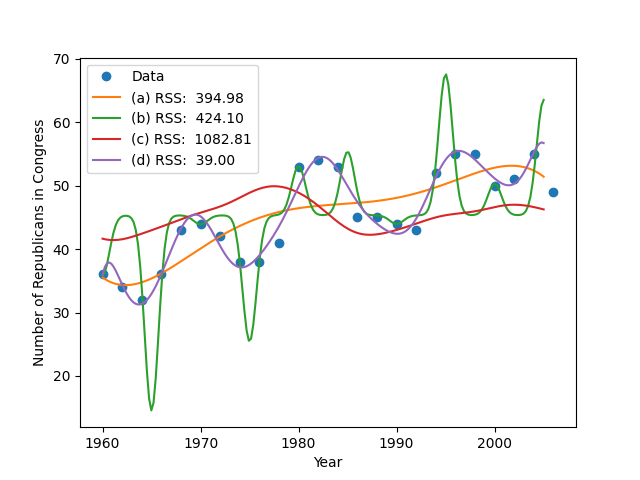
\includegraphics[scale=0.8]{P4_1}
\centering
\end{figure}

\newpage
\item The following plot is made in T1\_P4.

\begin{figure}[h]
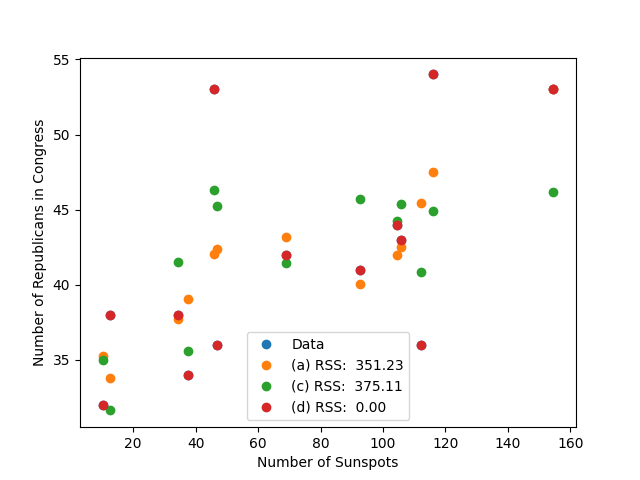
\includegraphics[scale=0.8]{P4_2}
\centering
\end{figure}

In this graph, the data is eclipsed by the third fit. The best fit for this 
model is the one made using basis (d). Despite the perfect fit, this model
is very generalizable at all. I do not believe the number of sunspots controls
the number of Republicans in the senate.

\end{enumerate}


\newpage
%%%%%%%%%%%%%%%%%%%%%%%%%%%%%%%%%%%%%%%%%%%%%
% Name and Calibration
%%%%%%%%%%%%%%%%%%%%%%%%%%%%%%%%%%%%%%%%%%%%%
\subsection*{Name}

Rodney Lafuente Mercado

\subsection*{Collaborators and Resources}
Whom did you work with, and did you use any resources beyond cs181-textbook and your notes?

I worked on my own and used python library documentation for pandas and numpy.


\subsection*{Calibration}
Approximately how long did this homework take you to complete (in hours)? 

Roughly 10 hours.

\end{document}